%%%%%%%%%%%%%%%%%%%%%%%%%%%%%%%%%%%%%%%%%%%%%%%%%%%%%%%
\subsubsection{Unpolarized PDFs}

\subsubsection*{General framework}

We express the collinear unpolarized PDFs as $f_{i}(x,\mu)$
where the index $i$ represents the parton flavor $i=\{g,u,\bar{u},d,\bar{d},s,\bar{s},...\}$,
$x$ is the fractional momentum carried by the parton, and $\mu$
is the factorization  scale.\footnote{We could add an additional index to specify the particular hadron
(proton, neutron, pion, nuclei, ...); as we mainly refer to the proton
  in this work, we will omit such a designation unless necessary.}
%
The value of $\mu$ is usually chosen to be the typical scale of the hard scattering
process involving the PDFs.
%
The PDF is a scheme-dependent quantity, and we typically work in
the $\overline{\rm MS}$ scheme; when this is convoluted with an appropriate
hard cross section (Wilson coefficient), we obtain a scheme-independent
physical observable (up to subleading terms in the perturbative expansion). 


The unpolarized PDFs appear in the factorization formulae for both inclusive DIS and hadroproduction processes. Namely, the DIS structure functions are given by
\begin{equation}
F_i(x,Q^2)=x\sum_a \int_x^1 \frac{{\rm d}z}{z}\,C_{i,a}\left(\frac{x}{z},\alpha_S(Q^2)\right)f_a(z,Q^2)\, ,
\end{equation}
where $x=\frac{Q^2}{2p\cdot q}$ is the standard Bjorken variable, given in terms of the momenta $q$ of the virtual photon ($q^2=-Q^2$), and $p$ of the proton. 
%
The hard coefficient functions $C_{i,a}$ can be computed perturbatively as an expansion in $\alpha_S$.
%
For the hadroproduction of an object $X$ in $pp$ collisions we have
\begin{equation}
  \label{eq:LHCxsec}
\sigma_{pp\to X}=\sum_{a,b}\int {\rm d}x_1 {\rm d}x_2\, f_a(x_1,\mu_F^2)f_b(x_2,\mu_F^2)\,\hat{\sigma}_{ab\to X}(x_1,x_2,s;\mu_{F},\mu_R)\;,
\end{equation}
where the hard cross section $\hat{\sigma}$ can again be calculated perturbatively. The $x_i$ are related to the kinematics of the final state.
%
In particular, at leading order it can be shown that
\be
x_{1,2}=\frac{M_X}{\sqrt{s}}e^{\pm y_X} \, ,
\ee
where $M_X$, $y_X$ are the invariant mass and rapidity of the produced system respectively.
%
The factorization and renormalization scales, $\mu_F$ and $\mu_R$, are taken to be of order the hard scale, $\mu_F,\mu_R
\sim Q$, of the process.

While the PDFs themselves cannot be calculated using perturbative methods, their dependence on the scale $\mu$ can be, and is given by the  
DGLAP evolution equations~\cite{Dokshitzer:1977sg,Gribov:1972ri,Altarelli:1977zs},
a set of integro-differential coupled equations of the form
\begin{equation}
  \label{eq:dglap}
\frac{\partial f_i(x,\mu^2)}{\partial \ln \mu^2}=\sum_{j=g,q,\bar{q}}\int_x^1 \frac{{\rm d}z}{z}P_{ij}(x/z)f_j(z,\mu^2)\;,
\end{equation}
Here, the logarithmic derivative of the PDF is determined by a convolution
of the PDFs with the DGLAP kernel $P_{ij}$ which can be computed
perturbatively in powers of $\alpha_{s}(\mu)$; $P_{ij}$ is known
to NNLO.\footnote{The DGLAP (Dokshitzer\textendash Gribov\textendash Lipatov\textendash Altarelli\textendash Parisi)
evolution can be modified by $\ln(1/x)$ terms at small-$x$, and
this is characterized by the BFLK (Balitsky-FadinKuraev-Lipatov) equations~\cite{Kuraev:1976ge,Kuraev:1977fs,Balitsky:1978ic}.
%
Additionally, at large-$x$ and small $\mu$ scale the above framework
can receive corrections from non-factorizeable higher-twist (HT) corrections.} 
%When performing the global fit to the data, we use the DGLAP equations to combine data from different $\mu$ scales when constraining the PDFs. 

Thus, when performing a global fit, the PDFs can be parameterised at one arbitrary input scale $Q_0\sim 1$ GeV, and these are connected directly via (\ref{eq:dglap}) to the higher scales $\mu$ that are probed by the data.
This parameterisation takes the generic form
\begin{equation}\label{eq:pdffunc}
f_{i}(x,Q_0)\sim x^{a}(1-x)^{b}\:C(x)\quad.
\end{equation}
The $(1-x)^b$ term, with $b_{f}>0$, ensures that the PDFs vanish in the elastic $x\to 1$ limit, as we would expect on basic physical grounds. 
%Such a form is also expected from the quark counting rules~\cite{Brodsky:1973kr}. 
The $x^a$ form, which dominates at low $x$, is predicted from general Regge theory considerations, although in modern fits the value of the power itself is left free. The interpolating function $C(x)$ determines the behaviour of the PDFs away from the $x\to 0$ and 1 limits, where it tends to a constant value. This is assumed to be a smoothly varying function of $x$, for which a variety of choices have been made in PDF fits.

There are a few constraints we
can impose on the $x$-dependence of the PDFs at this point. Since
the proton has the quantum numbers of two up quarks and one down quark,
we have the following quark number sum rules given in terms of first
moments: 
%
\begin{eqnarray}
\int_{0}^{1}dx\ \left[u(x,\mu)-\bar{u}(x,\mu)\right] & =\left\langle 1\right\rangle _{u^{-}}= & 2\\
\int_{0}^{1}dx\ \left[d(x,\mu)-\bar{d}(x,\mu)\right] & =\left\langle 1\right\rangle _{d^{-}}= & 1\\
\int_{0}^{1}dx\ \left[s(x,\mu)-\bar{s}(x,\mu)\right] & =\left\langle 1\right\rangle _{s^{-}}= & 0
\end{eqnarray}
with similar results for the heavy quarks: $\left\langle 1\right\rangle _{c^{-}}=\left\langle 1\right\rangle _{b^{-}}=\left\langle 1\right\rangle _{t^{-}}=0$. Thus for these valence distributions we must have $a>-1$ for the exponents in
Eq.~(\ref{eq:pdffunc}) or these integrals will diverge.

The fractional momentum carried
by each parton flavor is given by the second moments: 
%
\begin{eqnarray}
\int_{0}^{1}dx\ x\ \left[u(x,\mu)\right] & = & \left\langle x\right\rangle _{u}\\
\int_{0}^{1}dx\ x\ \left[u(x,\mu)+\bar{u}(x,\mu)\right] & = & \left\langle x\right\rangle _{u^{+}}\ .
\end{eqnarray}
%
Here, $\left\langle x\right\rangle _{u}$ is the fractional momentum
carried by the up-quark, $\left\langle x\right\rangle _{u^{+}}$ is
the fractional momentum carried by the up-quark and anti-up-quark.
Since the total momentum of the proton must equal the momentum of
its constituents, we have the momentum sum rule constraint: 
%
\begin{eqnarray}\label{eq:mom}
1 & = & \left\langle x\right\rangle _{g}+\left\langle x\right\rangle _{u^{+}}+\left\langle x\right\rangle _{d^{+}}+\left\langle x\right\rangle _{s^{+}}+\left\langle x\right\rangle _{c^{+}}+\left\langle x\right\rangle _{b^{+}}+\left\langle x\right\rangle _{t^{+}}+...
\end{eqnarray}
%
where the ``...'' represents any other partonic components (such
as a photon). Thus for non--valence distributions, we must have $a>-2$ to avoid a divergent contribution to (\ref{eq:mom}); typically we have $-2<a<-1$ for such distributions, and therefore for small $x$ the number of soft partons is infinite, although the momentum fraction carried by them is of course not.

\subsubsection*{Fitting PDFs from hard-scattering data}

The global PDF fitting framework is based on a combination of three basic components:
\begin{itemize}
\item A broad set of input hard-scattering cross-sections from deep-inelastic
  scattering and proton-proton collisions, providing information on the PDFs
  over a wide range of $x$ and for different flavour combinations.
  %
  While traditional PDF fits were based mostly on DIS structure function and Drell-Yan
  and inclusive jet
  cross-sections, in the recent years many other processes have demonstrated
  their usefulness for constraining PDFs, from top-quark pair production~\cite{Czakon:2016olj}
  to the $p_T$ of the $Z$ bosons~\cite{Boughezal:2017nla}
  and $D$ meson production in the forward region~\cite{Gauld:2016kpd}.
  %
  In Fig.~\ref{fig:kinplot-report} we show the representative kinematical coverage in the
    $(x,Q^2)$ of the DIS and proton-proton hard-scattering measurements that are
    used as input in a global unpolarized PDF fit, in this case NNPDF3.1.
    %
    In order to facilitate visualization, different
    datasets have been clustered together into families of
    related processes.

  \item Theoretical calculations of DIS and hadronic cross-sections
    for the highest perturbative order available.
    %
    Currently this means NNLO for the QCD corrections and NLO
    for the electroweak and photon-induced effects.
    %
    Moreover, these calculations should be provided in
    a format such as the evaluation of the hadronic
    cross-sections Eq.~(\ref{eq:LHCxsec}) is not too burdensome
    from the computational point of view.
    %
    To bypass these limitations, a number of fast interfaces have
    been developed that allow the efficient calculation
    of NLO (and NNLO) fully differential hadronic cross-sections.
    %
    The exploitation of fast interfaces such as {\tt APPLgrid},
    {\tt FastNLO} and {\tt aMCfast} is of utmost importance
    for modern PDF fits given the wealth of collider data used.

  \item A fitting methodology that determines the best-fit
    PDF parameters and their uncertainty from the minimization
    of a suitable statistical estimator, typically the $\chi^2$
    or a related estimator.
    %
    There are different alternative definitions of the $\chi^2$
    to be used in the global fit, for instance one frequently
    used definition is
    \begin{equation}
\chi^2 = \sum_{i,j}^{N_{\rm dat}} (T_i - D_i) ({\rm cov^{-1}})_{ij} (T_j - D_j),
\label{eq:chi2}
    \end{equation}
    where $N_{\rm dat}$ is the number of data points of a given experiment,
    and $T_i$ and $D_i$ are the corresponding theoretical calculations
    and the central values of the experimental data, respectively.
    %
    The theoretical predictions $D_i$ depend on the input
    PDF parametrization and thus on the fitting parameters.
    %
    Eq~(\ref{eq:chi2}) is therefore used as a  figure of merit to
    assess the agreement between theory
    and data.
    %
    The covariance matrix $({\rm cov})_{ij}$
    accounts for the various sources of experimental
    systematic uncertainties and
    also accepts several
    different definitions.
    %
    One example is the so-called
 $t_{0}$-prescription~\cite{Ball:2009qv}, 
where a fixed theory prediction $T_{i}^{(0)}$
is used to define the  contribution to the $\chi^2$
from the multiplicative systematic uncertainties, namely
\be
\label{eq:covmat_t00}
({\rm cov})_{ij}=
\delta_{ij} \sigma_{\rm stat}^2 + 
\sum_{\alpha=1}^{N_c}\sigma^{(c)}_{i,\alpha}\sigma^{(c)}_{j,\alpha}D_{i} D_{j}
+ \sum_{\beta=1}^{N_{\cal L}} \sigma_{i,\beta}^{({\cal L})}\sigma_{j,\beta}^{({\cal L})}
T^{(0)}_{i} T^{(0)}_{j}\, ,
\ee
where $\sigma_{\rm stat}$ is the uncorrelated uncertainty,
and $\sigma^{(c)}_{i,\alpha}$ ($\sigma^{(\cal L)}_{i,\beta}$)
are the additive (multiplicative) systematic uncertainties.
    
\end{itemize}
The goal of a global PDF fit is therefore to combine together
the best data and theory available in order to determine
the best-fit shape of the PDFs and the associated
uncertainties by means of the minimization
of the $\chi^2$ estimator Eq.~(\ref{eq:chi2}).

%%%%%%%%%%%%%%%%%%%%%%%%%%%%%%%%%%%%%%%%%%%%%%%%%%%%%%%%%%%%%%%%%%%%%
\begin{figure}[t]
\begin{center}
  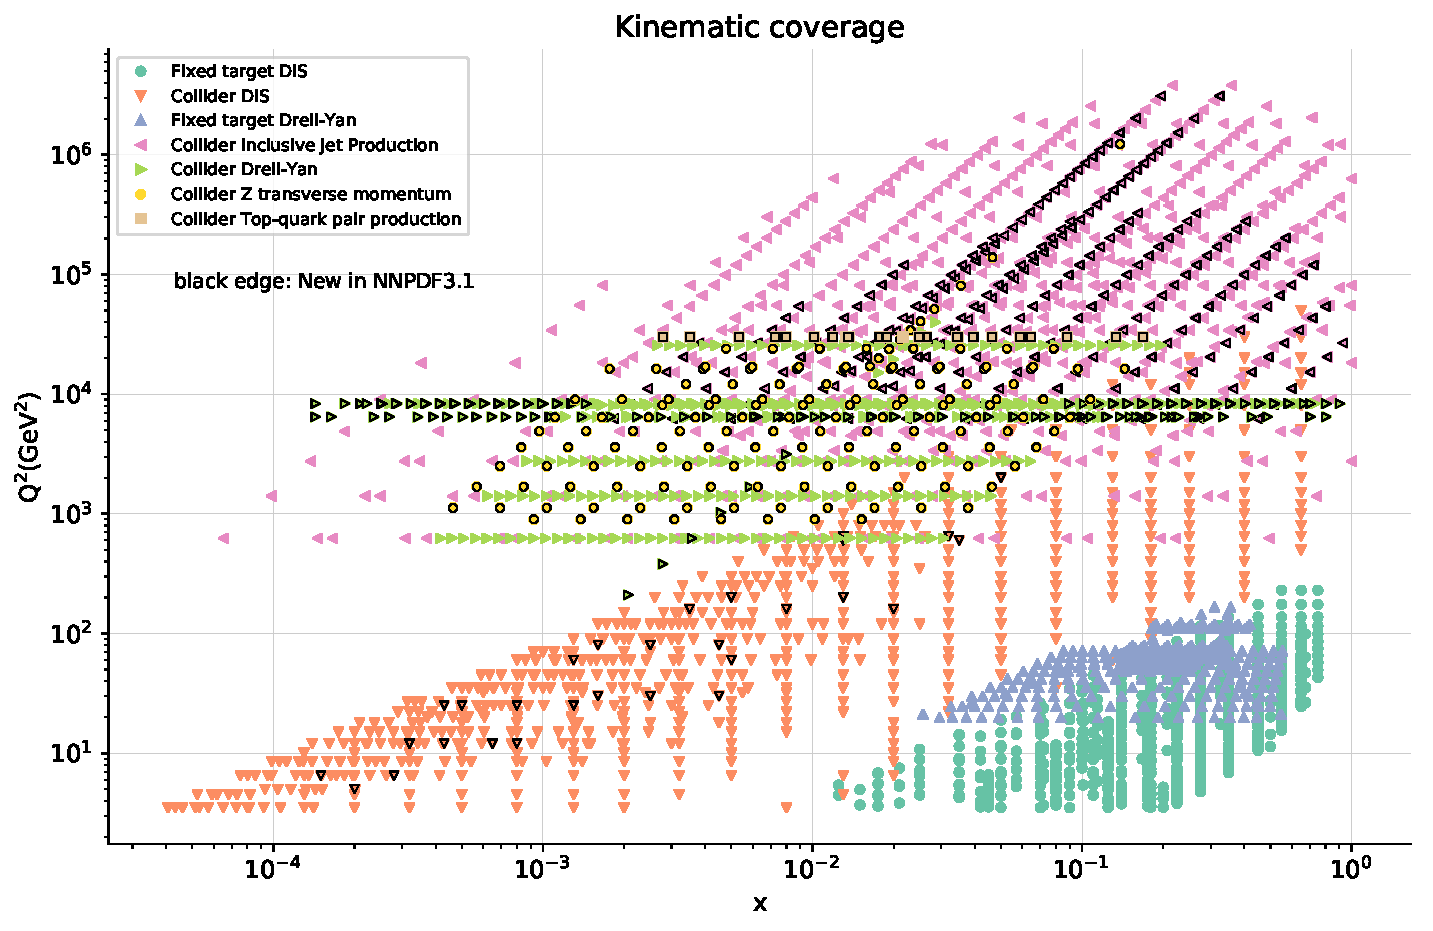
\includegraphics[scale=0.60]{plots/kinplot-report.pdf}
  \caption{\small Representative kinematical coverage in the
    $(x,Q^2)$ of the DIS and proton-proton hard-scattering measurements that are
    used as input in a global unpolarized PDF fit, in this case NNPDF3.1.
    %
    In order to facilitate visualization, different
    datasets have been clustered together into families of
    related processes.
    \label{fig:kinplot-report} 
  }
\end{center}
\end{figure}
%%%%%%%%%%%%%%%%%%%%%%%%%%%%%%%%%%%%%%%%%%%%%%%%%%%%%%%%%%%%%%%%%%%%%

A central ingredient of the global PDF fitting framework is the determination
of the various sources of experimental, theoretical and
methodological uncertainties that affect the best-fit PDFs.
%
In this respect,
there are two main methods to determine PDF uncertainties, the {\it
  Hessian} and the {\it Monte Carlo} methods, which we briefly
review now:
\begin{itemize}
\item The {\it Hessian method} is based on the parabolic
expansion of the $\chi^2$ in the vicinity of the minimum, parametrized
by a number of orthogonal eigenvectors within some fixed tolerance.
%
The basic idea of this method is that
in the vicinity of this minimum, the $\chi^2$ can
be approximated in terms of a quadratic expansion,
\be
\label{eq:hessianexpansion}
\Delta\chi^2 \equiv \chi^2- \chi^2_{\rm min}
=\sum_{i,j=1}^{n_{\rm par}}H_{ij}\lp a_i-a_i^0\rp
\lp a_j-a_j^0\rp \, ,
\ee
where the $n_{\rm par}$ PDF fit parameters are denoted by $\{a_1,\ldots,
a_{n_{\rm par}}\}$, and the best-fit values that minimize the
$\chi^2$ are indicated by
$\{a_1^0,\ldots,
a^0_{n_{\rm par}}\}$,
and the Hessian matrix is defined as
\be
H_{ij}\equiv \frac{1}{2} \frac{\partial^2\chi^2}{\partial a_i
\partial a_j}\Bigg|_{\{\vec{a}\}=
\{\vec{a^0}\}} \, .
\ee
By diagonalizing this Hessian matrix,
it is possible
to represent
PDF uncertainties in terms of orthogonal eigenvectors,
which then can be used to estimate the PDF uncertainty
for arbitrary cross-sections, using the master formula
of Hessian PDF sets for the uncertainty of the cross-section
$\mathcal{F}$, namely
\be
\label{eq:hessianmaster2}
\sigma_{\mathcal{F}}=\frac{1}{2}\lp \sum_{i,j}^{n_{\rm par}}
\lc \mathcal{F}(S_i^+)-\mathcal{F}(S_i^-) \rc \rp^{1/2} \, ,
\ee
where $S_i^{\pm}$ correspond to the $i$-th eigenvector
associated to positive and negative variations with respect
to the best fit value.

\item The {\it Monte Carlo method} is based instead
  on constructing a representation
  of the probability distribution of the experimental data in terms
  of a large number  $N_{\rm rep}$ of {\it replicas}, and then
PDF fits are then performed separately on each of these Monte Carlo replicas.
%
The resulting ensemble of PDFs represents the probability density in the space
of parton distributions.
%
This requires generating a large number of artificial replicas
of the original data which encode the same information on
central values, variances and correlations as that provided by the experiments.
%
In particular, given an experimental measurement of a hard-scattering
cross-section denoted generically by $F_{I}^{\rm (exp)}$ with
total uncorrelated uncertainty $\sigma_{I}^{\rm (stat)}$, $N_{\rm sys}$ fully
correlated systematic uncertainties $\sigma^{\rm (corr)}_{I,c}$ and
$N_a$ ($N_r$) absolute (relative) normalization uncertainties
$\sigma^{\rm (norm)}_{I,n}$, the artificial
MC replicas are constructed using the following expression
\be
\label{eq:replicas}
F_{I}^{(\art)(k)}=S_{I,N}^{(k)} F_{I}^{\rm (\mrexp)}\lp 1+
 \sum_{c=1}^{N_{\rm sys}}r_{I,c}^{(k)}\sigma^{\rm (corr)}_{I,c}+r_{I}^{(k)}\sigma_{I}^{\rm (stat)}\rp
 \ , \quad k=1,\ldots,N_{\rep} \ ,
\ee
where $S_{I,N}^{(k)}$ is the the normalization prefactor.
%
Here the variables $r_{I,c}^{(k)},r_{I}^{(k)},r_{p,n}^{(k)}$ are
 univariate gaussian random numbers.
 %
 For each replica the random fluctuations
 associated to a given fully correlated systematic
 uncertainty will be the same
 for all data points, $r^{(k)}_{I,c}=r^{(k)}_{I',c}$.
 %
 In the Monte Carlo method, the expectation function of a generic
cross-section $ \mathcal{F} [ \{  q \}]$
is evaluated as an average over the replica sample,
\be
\label{masterave}
\la \mathcal{F} [ \{  q \}] \ra
= \frac{1}{N_{\rm rep}} \sum_{k=1}^{N_{\rm set}}
\mathcal{F} [ \{  q^{(k)} \}] \, ,
\ee
and the corresponding uncertainty is then determined as the variance of the
Monte Carlo sample,
\be
\sigma_{\mathcal{F}} =
\left( \frac{1}{N_{\rm rep}-1}
\sum_{k=1}^{N_{\rm rep}}   
\lp \mathcal{F} [ \{  q^{(k)} \}] 
-   \la \mathcal{F} [ \{  q \}] \ra\rp^2 
 \right)^{1/2}.
\label{mastersig}
\ee

\end{itemize}

In the rest of this document, when comparing the results of global PDF fits
with the results of lattice QCD calculations we will use Eqns.~(\ref{eq:hessianmaster2}) and~(\ref{mastersig})
to evaluate the PDF uncertainties of Hessian and Monte Carlo PDF sets, respectively.

\subsubsection{State-of-the-art global PDF fits}

Various collaborations provide regular updates of their global unpolarized
PDF fits.
%
The latest fits from the three major global fitting collaborations, CT14~\cite{Dulat:2015mca}, MMHT14~\cite{Harland-Lang:2014zoa} and NNPDF3.1 are performed up to NNLO in the strong coupling, and include data from the HERA $e^{\pm} p$ collider, fixed (nuclear and proton) target experiments, the Tevatron $p\overline{p}$ collider and the LHC. 
%
The ABMP16~\cite{Alekhin:2017kpj} set fits to a similar global data set, but differs in its treatment of errors and heavy flavours (see below). The HERAPDF2.0~\cite{Abramowicz:2015mha} set fits to the final combined HERA Run I + II data set only, with the aim of determining the PDFs from a completely consistent DIS data sample; in $x$ regions which are less constrained by HERA data, the uncertainties can be quite large. The CJ15~\cite{Accardi:2016qay} NLO set focuses on constraining the PDFs at higher $x$ by lowering $Q^2$ and $W^2$ cuts in DIS. This greatly increases the available data, but requires additional modelling of power--like $\sim 1/Q^2$ corrections.

As described above, to perform a fit, some form for the interpolating function $C(x)$ in (\ref{eq:pdffunc}) must be assumed. The simplest ansatz, which has been very widely used, is to take a basic polynomial form in $x$ (or $\sqrt{x}$), such as
\begin{equation}\label{eq:lpower}
C(x)=1+c\sqrt{x}+d x+...\;.
\end{equation}
Forms of this type are for example taken by CJ, HERAPDF and earlier MMHT and CT sets. More recently, the CT and MMHT collaborations instead expand in terms of a basis of  Bernstein and Chebyshev polynomials, respectively.
%
While formally equivalent to the simply polynomial expansion (\ref{eq:lpower}), these are much more convenient for fitting as the number of free parameters $n$ is increased. In the latest sets, there are $O(20-40)$ free parameters in total.
%
An alternative approach is taken by the NNPDF collaboration. Here, the interpolating function is modeled with a multi--layer feed forward neural network. In practice, this allows for a greatly increased number of free parameters, typically $\sim$ an order of magnitude higher than other sets. The form of (\ref{eq:pdffunc}) is still assumed, but these are pre--processing factors that speed up the minimisation procedure but which do not in principle have to be explicitly included. 
